% Options for packages loaded elsewhere
\PassOptionsToPackage{unicode}{hyperref}
\PassOptionsToPackage{hyphens}{url}
\PassOptionsToPackage{dvipsnames,svgnames,x11names}{xcolor}
%
\documentclass[
  12pt,
  letterpaper,
  DIV=11,
  numbers=noendperiod]{scrartcl}

\usepackage{amsmath,amssymb}
\usepackage{iftex}
\ifPDFTeX
  \usepackage[T1]{fontenc}
  \usepackage[utf8]{inputenc}
  \usepackage{textcomp} % provide euro and other symbols
\else % if luatex or xetex
  \usepackage{unicode-math}
  \defaultfontfeatures{Scale=MatchLowercase}
  \defaultfontfeatures[\rmfamily]{Ligatures=TeX,Scale=1}
\fi
\usepackage{lmodern}
\ifPDFTeX\else  
    % xetex/luatex font selection
\fi
% Use upquote if available, for straight quotes in verbatim environments
\IfFileExists{upquote.sty}{\usepackage{upquote}}{}
\IfFileExists{microtype.sty}{% use microtype if available
  \usepackage[]{microtype}
  \UseMicrotypeSet[protrusion]{basicmath} % disable protrusion for tt fonts
}{}
\makeatletter
\@ifundefined{KOMAClassName}{% if non-KOMA class
  \IfFileExists{parskip.sty}{%
    \usepackage{parskip}
  }{% else
    \setlength{\parindent}{0pt}
    \setlength{\parskip}{6pt plus 2pt minus 1pt}}
}{% if KOMA class
  \KOMAoptions{parskip=half}}
\makeatother
\usepackage{xcolor}
\usepackage[top=1.5cm, bottom=1.5cm, left=2cm, right=2cm]{geometry}
\setlength{\emergencystretch}{3em} % prevent overfull lines
\setcounter{secnumdepth}{-\maxdimen} % remove section numbering
% Make \paragraph and \subparagraph free-standing
\ifx\paragraph\undefined\else
  \let\oldparagraph\paragraph
  \renewcommand{\paragraph}[1]{\oldparagraph{#1}\mbox{}}
\fi
\ifx\subparagraph\undefined\else
  \let\oldsubparagraph\subparagraph
  \renewcommand{\subparagraph}[1]{\oldsubparagraph{#1}\mbox{}}
\fi

\usepackage{color}
\usepackage{fancyvrb}
\newcommand{\VerbBar}{|}
\newcommand{\VERB}{\Verb[commandchars=\\\{\}]}
\DefineVerbatimEnvironment{Highlighting}{Verbatim}{commandchars=\\\{\}}
% Add ',fontsize=\small' for more characters per line
\usepackage{framed}
\definecolor{shadecolor}{RGB}{241,243,245}
\newenvironment{Shaded}{\begin{snugshade}}{\end{snugshade}}
\newcommand{\AlertTok}[1]{\textcolor[rgb]{0.68,0.00,0.00}{#1}}
\newcommand{\AnnotationTok}[1]{\textcolor[rgb]{0.37,0.37,0.37}{#1}}
\newcommand{\AttributeTok}[1]{\textcolor[rgb]{0.40,0.45,0.13}{#1}}
\newcommand{\BaseNTok}[1]{\textcolor[rgb]{0.68,0.00,0.00}{#1}}
\newcommand{\BuiltInTok}[1]{\textcolor[rgb]{0.00,0.23,0.31}{#1}}
\newcommand{\CharTok}[1]{\textcolor[rgb]{0.13,0.47,0.30}{#1}}
\newcommand{\CommentTok}[1]{\textcolor[rgb]{0.37,0.37,0.37}{#1}}
\newcommand{\CommentVarTok}[1]{\textcolor[rgb]{0.37,0.37,0.37}{\textit{#1}}}
\newcommand{\ConstantTok}[1]{\textcolor[rgb]{0.56,0.35,0.01}{#1}}
\newcommand{\ControlFlowTok}[1]{\textcolor[rgb]{0.00,0.23,0.31}{#1}}
\newcommand{\DataTypeTok}[1]{\textcolor[rgb]{0.68,0.00,0.00}{#1}}
\newcommand{\DecValTok}[1]{\textcolor[rgb]{0.68,0.00,0.00}{#1}}
\newcommand{\DocumentationTok}[1]{\textcolor[rgb]{0.37,0.37,0.37}{\textit{#1}}}
\newcommand{\ErrorTok}[1]{\textcolor[rgb]{0.68,0.00,0.00}{#1}}
\newcommand{\ExtensionTok}[1]{\textcolor[rgb]{0.00,0.23,0.31}{#1}}
\newcommand{\FloatTok}[1]{\textcolor[rgb]{0.68,0.00,0.00}{#1}}
\newcommand{\FunctionTok}[1]{\textcolor[rgb]{0.28,0.35,0.67}{#1}}
\newcommand{\ImportTok}[1]{\textcolor[rgb]{0.00,0.46,0.62}{#1}}
\newcommand{\InformationTok}[1]{\textcolor[rgb]{0.37,0.37,0.37}{#1}}
\newcommand{\KeywordTok}[1]{\textcolor[rgb]{0.00,0.23,0.31}{#1}}
\newcommand{\NormalTok}[1]{\textcolor[rgb]{0.00,0.23,0.31}{#1}}
\newcommand{\OperatorTok}[1]{\textcolor[rgb]{0.37,0.37,0.37}{#1}}
\newcommand{\OtherTok}[1]{\textcolor[rgb]{0.00,0.23,0.31}{#1}}
\newcommand{\PreprocessorTok}[1]{\textcolor[rgb]{0.68,0.00,0.00}{#1}}
\newcommand{\RegionMarkerTok}[1]{\textcolor[rgb]{0.00,0.23,0.31}{#1}}
\newcommand{\SpecialCharTok}[1]{\textcolor[rgb]{0.37,0.37,0.37}{#1}}
\newcommand{\SpecialStringTok}[1]{\textcolor[rgb]{0.13,0.47,0.30}{#1}}
\newcommand{\StringTok}[1]{\textcolor[rgb]{0.13,0.47,0.30}{#1}}
\newcommand{\VariableTok}[1]{\textcolor[rgb]{0.07,0.07,0.07}{#1}}
\newcommand{\VerbatimStringTok}[1]{\textcolor[rgb]{0.13,0.47,0.30}{#1}}
\newcommand{\WarningTok}[1]{\textcolor[rgb]{0.37,0.37,0.37}{\textit{#1}}}

\providecommand{\tightlist}{%
  \setlength{\itemsep}{0pt}\setlength{\parskip}{0pt}}\usepackage{longtable,booktabs,array}
\usepackage{calc} % for calculating minipage widths
% Correct order of tables after \paragraph or \subparagraph
\usepackage{etoolbox}
\makeatletter
\patchcmd\longtable{\par}{\if@noskipsec\mbox{}\fi\par}{}{}
\makeatother
% Allow footnotes in longtable head/foot
\IfFileExists{footnotehyper.sty}{\usepackage{footnotehyper}}{\usepackage{footnote}}
\makesavenoteenv{longtable}
\usepackage{graphicx}
\makeatletter
\def\maxwidth{\ifdim\Gin@nat@width>\linewidth\linewidth\else\Gin@nat@width\fi}
\def\maxheight{\ifdim\Gin@nat@height>\textheight\textheight\else\Gin@nat@height\fi}
\makeatother
% Scale images if necessary, so that they will not overflow the page
% margins by default, and it is still possible to overwrite the defaults
% using explicit options in \includegraphics[width, height, ...]{}
\setkeys{Gin}{width=\maxwidth,height=\maxheight,keepaspectratio}
% Set default figure placement to htbp
\makeatletter
\def\fps@figure{htbp}
\makeatother

\KOMAoption{captions}{tableheading}
\usepackage{graphicx}
\usepackage{fancyhdr}
\usepackage{wallpaper}
\usepackage{caption}
\usepackage{subcaption}
\makeatletter
\@ifpackageloaded{caption}{}{\usepackage{caption}}
\AtBeginDocument{%
\ifdefined\contentsname
  \renewcommand*\contentsname{Table of contents}
\else
  \newcommand\contentsname{Table of contents}
\fi
\ifdefined\listfigurename
  \renewcommand*\listfigurename{List of Figures}
\else
  \newcommand\listfigurename{List of Figures}
\fi
\ifdefined\listtablename
  \renewcommand*\listtablename{List of Tables}
\else
  \newcommand\listtablename{List of Tables}
\fi
\ifdefined\figurename
  \renewcommand*\figurename{Figure}
\else
  \newcommand\figurename{Figure}
\fi
\ifdefined\tablename
  \renewcommand*\tablename{Table}
\else
  \newcommand\tablename{Table}
\fi
}
\@ifpackageloaded{float}{}{\usepackage{float}}
\floatstyle{ruled}
\@ifundefined{c@chapter}{\newfloat{codelisting}{h}{lop}}{\newfloat{codelisting}{h}{lop}[chapter]}
\floatname{codelisting}{Listing}
\newcommand*\listoflistings{\listof{codelisting}{List of Listings}}
\makeatother
\makeatletter
\makeatother
\makeatletter
\@ifpackageloaded{caption}{}{\usepackage{caption}}
\@ifpackageloaded{subcaption}{}{\usepackage{subcaption}}
\makeatother
\ifLuaTeX
  \usepackage{selnolig}  % disable illegal ligatures
\fi
\usepackage{bookmark}

\IfFileExists{xurl.sty}{\usepackage{xurl}}{} % add URL line breaks if available
\urlstyle{same} % disable monospaced font for URLs
\hypersetup{
  colorlinks=true,
  linkcolor={blue},
  filecolor={Maroon},
  citecolor={Blue},
  urlcolor={Blue},
  pdfcreator={LaTeX via pandoc}}

\author{}
\date{Invalid Date}

\begin{document}

\begin{titlepage}
\centering

\begin{minipage}[c]{6cm}
    \centering
    
\includegraphics[width=\linewidth]{Logo.png}
\end{minipage}
\hspace{1cm}
\begin{minipage}[c]{6cm}
    \centering
    
\includegraphics[width=\linewidth]{ssd_logo_couleur_noir_variante_biostats.png}
\end{minipage}

\vspace{0.5cm}

{\scshape\LARGE Université de Montpellier \par}
\vspace{1cm}
{\scshape\Large Apprentissage statistique \par}
\vspace{0.5cm}
\rule{\linewidth}{0.5 mm} \\[0.4 cm]
{\huge\bfseries  TP 3: SVM \par}
\rule{\linewidth}{0.5 mm} \\[1.5 cm]

% Élève et encadrante
\begin{minipage}{0.5\textwidth}
\begin{flushleft} \large
\emph{\textbf{Élève :}}\\
Labourail Célia
\end{flushleft}
\end{minipage}
~
\begin{minipage}{0.4\textwidth}
\begin{flushright} \large
\emph{\textbf{Encadrante :}} \\
B.Bensaid
\end{flushright}
\end{minipage}

\vspace*{\fill}

% Date
\begin{center}
{\today}
\end{center}

\end{titlepage}

\section{Introduction}\label{introduction}

\begin{Shaded}
\begin{Highlighting}[]
\ImportTok{import}\NormalTok{ numpy }\ImportTok{as}\NormalTok{ np}
\ImportTok{import}\NormalTok{ matplotlib.pyplot }\ImportTok{as}\NormalTok{ plt}
\ImportTok{from}\NormalTok{ sklearn.svm }\ImportTok{import}\NormalTok{ SVC}

\ImportTok{from}\NormalTok{ svm\_source }\ImportTok{import} \OperatorTok{*}
\ImportTok{from}\NormalTok{ sklearn }\ImportTok{import}\NormalTok{ svm}
\ImportTok{from}\NormalTok{ sklearn }\ImportTok{import}\NormalTok{ datasets}
\ImportTok{from}\NormalTok{ sklearn.utils }\ImportTok{import}\NormalTok{ shuffle}
\ImportTok{from}\NormalTok{ sklearn.preprocessing }\ImportTok{import}\NormalTok{ StandardScaler}
\ImportTok{from}\NormalTok{ sklearn.model\_selection }\ImportTok{import}\NormalTok{ train\_test\_split, GridSearchCV}
\ImportTok{from}\NormalTok{ sklearn.datasets }\ImportTok{import}\NormalTok{ fetch\_lfw\_people}
\ImportTok{from}\NormalTok{ sklearn.decomposition }\ImportTok{import}\NormalTok{ PCA}
\ImportTok{from}\NormalTok{ time }\ImportTok{import}\NormalTok{ time}

\NormalTok{scaler }\OperatorTok{=}\NormalTok{ StandardScaler()}

\ImportTok{import}\NormalTok{ warnings}
\NormalTok{warnings.filterwarnings(}\StringTok{"ignore"}\NormalTok{)}

\NormalTok{plt.style.use(}\StringTok{\textquotesingle{}ggplot\textquotesingle{}}\NormalTok{)}
\end{Highlighting}
\end{Shaded}

\begin{Shaded}
\begin{Highlighting}[]
\CommentTok{\#\#\#\#\#\#\#\#\#\#\#\#\#\#\#\#\#\#\#\#\#\#\#\#\#\#\#\#\#\#\#\#\#\#\#\#\#\#\#\#\#\#\#\#\#\#\#\#\#\#\#\#\#\#\#\#\#\#\#\#\#\#\#\#\#\#\#\#\#\#\#\#\#\#\#\#\#\#\#}
\CommentTok{\#               Toy dataset : 2 gaussians}
\CommentTok{\#\#\#\#\#\#\#\#\#\#\#\#\#\#\#\#\#\#\#\#\#\#\#\#\#\#\#\#\#\#\#\#\#\#\#\#\#\#\#\#\#\#\#\#\#\#\#\#\#\#\#\#\#\#\#\#\#\#\#\#\#\#\#\#\#\#\#\#\#\#\#\#\#\#\#\#\#\#\#}

\NormalTok{n1 }\OperatorTok{=} \DecValTok{200}
\NormalTok{n2 }\OperatorTok{=} \DecValTok{200}
\NormalTok{mu1 }\OperatorTok{=}\NormalTok{ [}\FloatTok{1.}\NormalTok{, }\FloatTok{1.}\NormalTok{]}
\NormalTok{mu2 }\OperatorTok{=}\NormalTok{ [}\OperatorTok{{-}}\FloatTok{1.}\OperatorTok{/}\DecValTok{2}\NormalTok{, }\OperatorTok{{-}}\FloatTok{1.}\OperatorTok{/}\DecValTok{2}\NormalTok{]}
\NormalTok{sigma1 }\OperatorTok{=}\NormalTok{ [}\FloatTok{0.9}\NormalTok{, }\FloatTok{0.9}\NormalTok{]}
\NormalTok{sigma2 }\OperatorTok{=}\NormalTok{ [}\FloatTok{0.9}\NormalTok{, }\FloatTok{0.9}\NormalTok{]}
\NormalTok{X1, y1 }\OperatorTok{=}\NormalTok{ rand\_bi\_gauss(n1, n2, mu1, mu2, sigma1, sigma2)}

\NormalTok{plt.show()}
\NormalTok{plt.close(}\StringTok{"all"}\NormalTok{)}
\NormalTok{plt.ion()}
\NormalTok{plt.figure(}\DecValTok{1}\NormalTok{, figsize}\OperatorTok{=}\NormalTok{(}\DecValTok{15}\NormalTok{, }\DecValTok{5}\NormalTok{))}
\NormalTok{plt.title(}\StringTok{\textquotesingle{}First data set\textquotesingle{}}\NormalTok{)}
\NormalTok{plot\_2d(X1, y1)}

\NormalTok{X\_train }\OperatorTok{=}\NormalTok{ X1[::}\DecValTok{2}\NormalTok{]}
\NormalTok{Y\_train }\OperatorTok{=}\NormalTok{ y1[::}\DecValTok{2}\NormalTok{].astype(}\BuiltInTok{int}\NormalTok{)}
\NormalTok{X\_test }\OperatorTok{=}\NormalTok{ X1[}\DecValTok{1}\NormalTok{::}\DecValTok{2}\NormalTok{]}
\NormalTok{Y\_test }\OperatorTok{=}\NormalTok{ y1[}\DecValTok{1}\NormalTok{::}\DecValTok{2}\NormalTok{].astype(}\BuiltInTok{int}\NormalTok{)}

\CommentTok{\# fit the model with linear kernel}
\NormalTok{clf }\OperatorTok{=}\NormalTok{ SVC(kernel}\OperatorTok{=}\StringTok{\textquotesingle{}linear\textquotesingle{}}\NormalTok{)}
\NormalTok{clf.fit(X\_train, Y\_train)}

\CommentTok{\# predict labels for the test data base}
\NormalTok{y\_pred }\OperatorTok{=}\NormalTok{ clf.predict(X\_test)}

\CommentTok{\# check your score}
\NormalTok{score }\OperatorTok{=}\NormalTok{ clf.score(X\_test, Y\_test)}
\BuiltInTok{print}\NormalTok{(}\StringTok{\textquotesingle{}Score : }\SpecialCharTok{\%s}\StringTok{\textquotesingle{}} \OperatorTok{\%}\NormalTok{ score)}

\CommentTok{\# display the frontiere}
\KeywordTok{def}\NormalTok{ f(xx):}
    \CommentTok{"""Classifier: needed to avoid warning due to shape issues"""}
    \ControlFlowTok{return}\NormalTok{ clf.predict(xx.reshape(}\DecValTok{1}\NormalTok{, }\OperatorTok{{-}}\DecValTok{1}\NormalTok{))}

\NormalTok{plt.figure()}
\NormalTok{frontiere(f, X\_train, Y\_train, w}\OperatorTok{=}\VariableTok{None}\NormalTok{, step}\OperatorTok{=}\DecValTok{50}\NormalTok{, alpha\_choice}\OperatorTok{=}\DecValTok{1}\NormalTok{)}

\CommentTok{\# Same procedure but with a grid search}
\NormalTok{parameters }\OperatorTok{=}\NormalTok{ \{}\StringTok{\textquotesingle{}kernel\textquotesingle{}}\NormalTok{: [}\StringTok{\textquotesingle{}linear\textquotesingle{}}\NormalTok{], }\StringTok{\textquotesingle{}C\textquotesingle{}}\NormalTok{: }\BuiltInTok{list}\NormalTok{(np.linspace(}\FloatTok{0.001}\NormalTok{, }\DecValTok{3}\NormalTok{, }\DecValTok{21}\NormalTok{))\}}
\NormalTok{clf2 }\OperatorTok{=}\NormalTok{ SVC()}
\NormalTok{clf\_grid }\OperatorTok{=}\NormalTok{ GridSearchCV(clf2, parameters, n\_jobs}\OperatorTok{=}\DecValTok{1}\NormalTok{)}
\NormalTok{clf\_grid.fit(X\_train, Y\_train)}

\CommentTok{\# check your score}
\BuiltInTok{print}\NormalTok{(clf\_grid.best\_params\_)}
\BuiltInTok{print}\NormalTok{(}\StringTok{\textquotesingle{}Score : }\SpecialCharTok{\%s}\StringTok{\textquotesingle{}} \OperatorTok{\%}\NormalTok{ clf\_grid.score(X\_test, Y\_test))}

\KeywordTok{def}\NormalTok{ f\_grid(xx):}
    \CommentTok{"""Classifier: needed to avoid warning due to shape issues"""}
    \ControlFlowTok{return}\NormalTok{ clf\_grid.predict(xx.reshape(}\DecValTok{1}\NormalTok{, }\OperatorTok{{-}}\DecValTok{1}\NormalTok{))}

\CommentTok{\# display the frontiere}
\NormalTok{plt.figure()}
\NormalTok{frontiere(f\_grid, X\_train, Y\_train, w}\OperatorTok{=}\VariableTok{None}\NormalTok{, step}\OperatorTok{=}\DecValTok{50}\NormalTok{, alpha\_choice}\OperatorTok{=}\DecValTok{1}\NormalTok{)}
\end{Highlighting}
\end{Shaded}

\begin{verbatim}
Score : 0.875
{'C': np.float64(0.3009), 'kernel': 'linear'}
Score : 0.875
\end{verbatim}

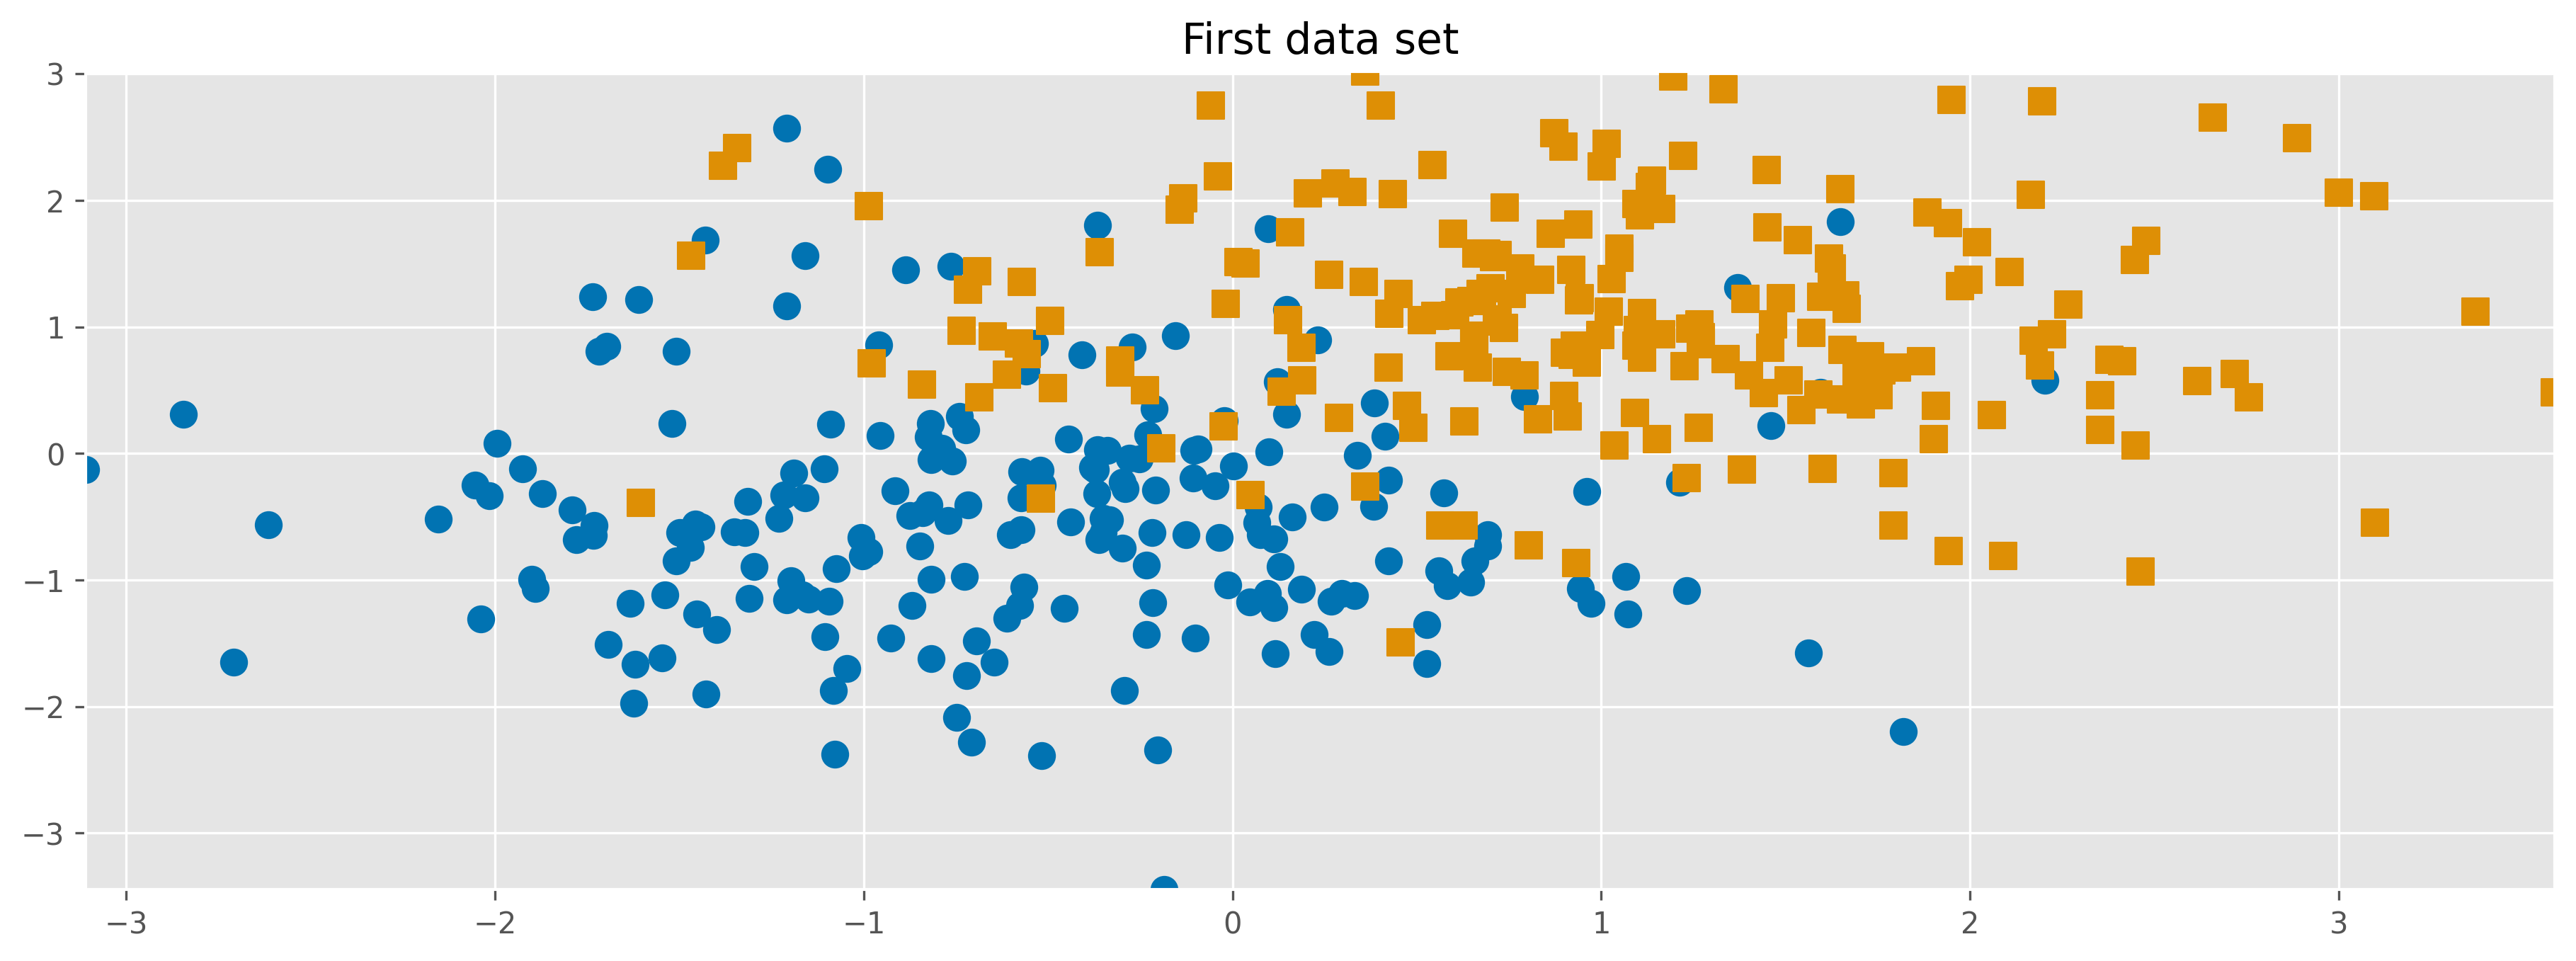
\includegraphics{Tp3_Celia_Labourail_files/figure-pdf/cell-3-output-2.png}

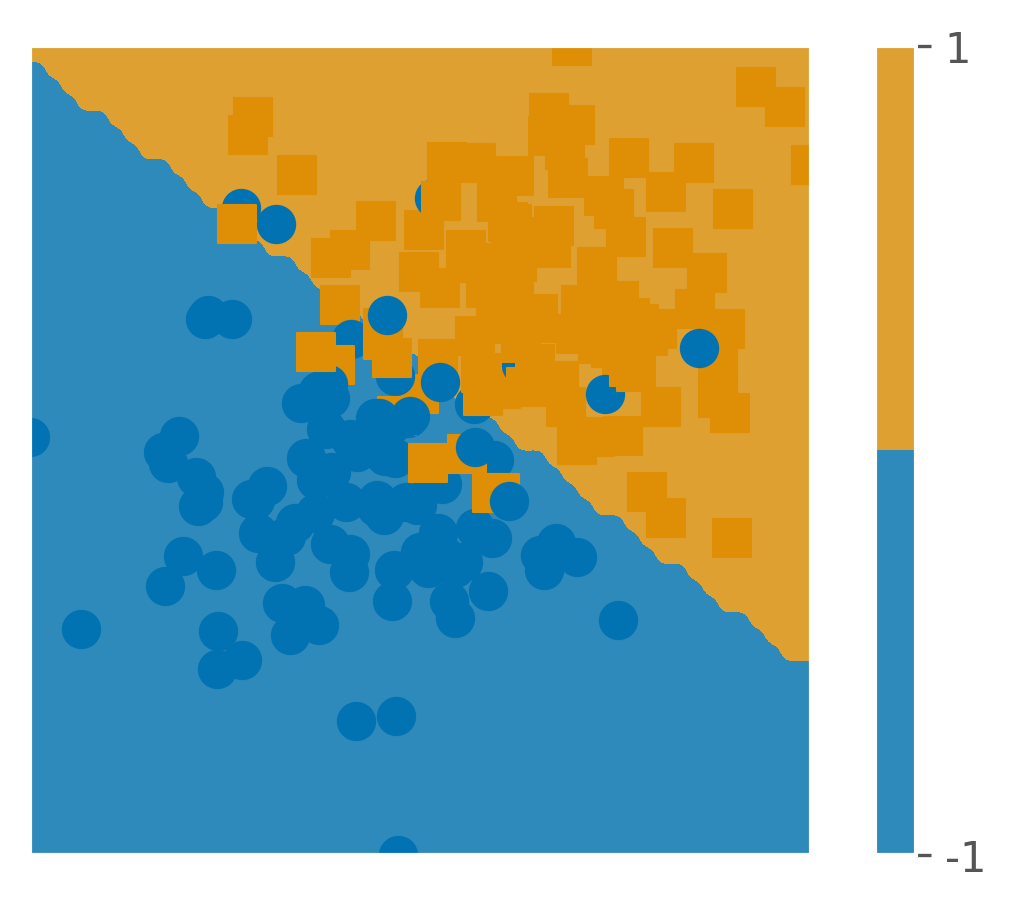
\includegraphics{Tp3_Celia_Labourail_files/figure-pdf/cell-3-output-3.png}

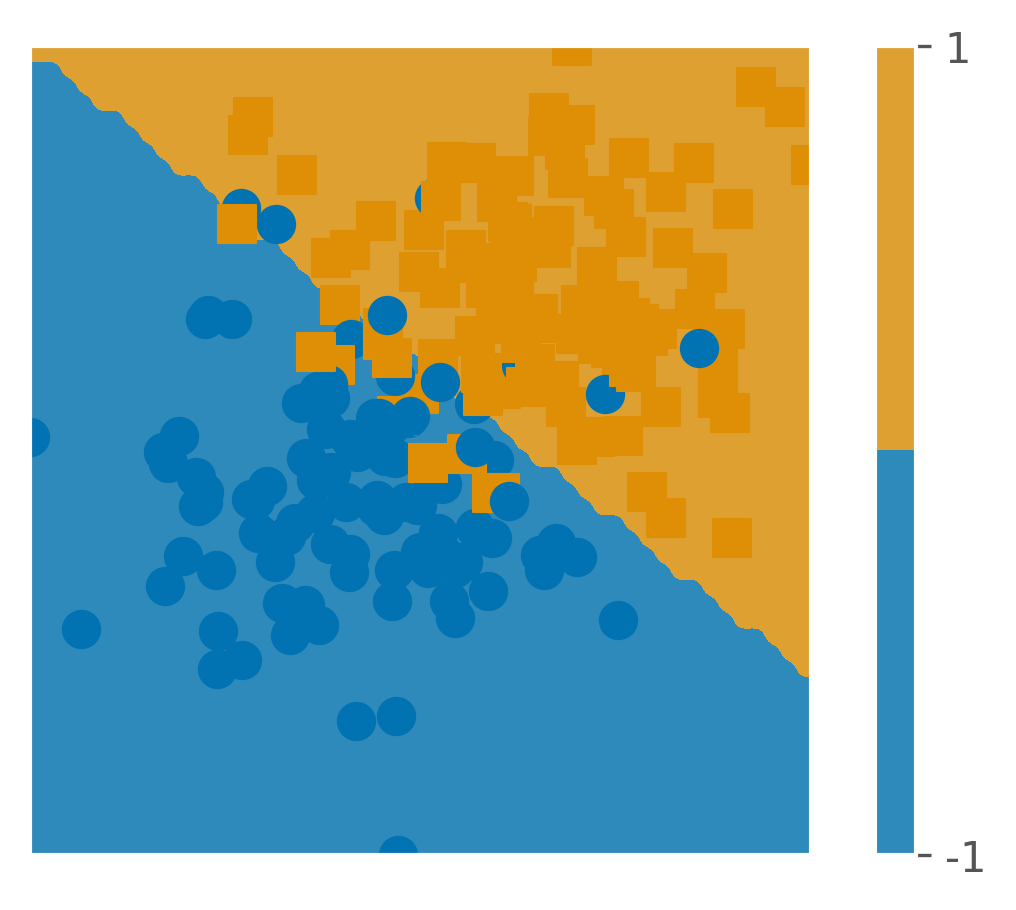
\includegraphics{Tp3_Celia_Labourail_files/figure-pdf/cell-3-output-4.png}



\end{document}
